\documentclass[12pt,a4paper]{article}

% ==================== PACKAGES ====================
\usepackage[utf8]{inputenc}
\usepackage[spanish]{babel}
\usepackage{geometry}
\usepackage{graphicx}
\usepackage{booktabs}
\usepackage{longtable}
\usepackage{array}
\usepackage{multirow}
\usepackage{amsmath}
\usepackage{amssymb}
\usepackage{hyperref}
\usepackage{float}
\usepackage{caption}
\usepackage{subcaption}
\usepackage{xcolor}
\usepackage{fancyhdr}
\usepackage{titlesec}
\usepackage{pgffor}
\usepackage{pdflscape}
\usepackage{chngcntr}
\counterwithin{table}{subsection}
\usepackage{graphicx}
\usepackage{float}
\usepackage{hyperref}
% ==================== PAGE SETUP ====================
\geometry{
	left=2.5cm,
	right=2.5cm,
	top=3cm,
	bottom=3cm
}

% ==================== HEADER & FOOTER ====================
\pagestyle{fancy}
\fancyhf{}
\fancyhead[L]{Análisis de rendimiento Futbolístico (2024)}
\fancyhead[R]{UCV - 2025}
\fancyfoot[C]{\thepage}

% ==================== HYPERLINKS ====================
\hypersetup{
	colorlinks=true,
	linkcolor=blue,
	filecolor=magenta,      
	urlcolor=cyan,
	citecolor=blue
}

% ==================== DOCUMENT ====================
\begin{document}
	
	% ==================== TITLE PAGE ====================
	\begin{titlepage}
		\centering
		
		\vspace*{1cm}
		
		% Universidad header
		{\Large\textbf{Universidad Central de Venezuela}}\\[0.3cm]
		{\large Facultad de Ciencias}\\[0.2cm]
		{\large Escuela de Matemáticas}\\[0.2cm]
		{\large Estadística}\\[0.5cm]
		
		\vspace{1cm}
		
		% Course info
		{\large Período Lectivo: 2 - 2025}\\[0.3cm]
		{\large Prof.: Orlian Prato}\\[2cm]
		
		% Title
		\rule{\linewidth}{0.5mm}\\[0.4cm]
		{\huge\bfseries Proyecto Nro.1}\\[0.2cm]
		{\Large\bfseries Análisis de Rendimiento Futbolístico 2024}\\[0.4cm]
		\rule{\linewidth}{0.5mm}\\[0.2cm]
		\begin{small}
		{comparativo entre equipos elite y equipos de mediano/bajo rendimiento}\\[2cm]
		\end{small}
		\vfill
		
		% Author info
		{\large Autor(es):}\\[0.3cm]
		{\large Chacón Kimberly}\\
		{\large C.I.: V-27.254.966}\\[0.1cm]
		{\large Guevara Anyeli}\\
		{\large C.I.: V-26.989.462}\\[2cm]
		\vfill
		
		% Date and location
		{\large Caracas, Venezuela}\\
		{\large \today}
		
	\end{titlepage}
	
	% ==================== PAGE ====================
	\newpage
	
	\vspace*{1cm}
	\begin{center}
	% Introducción header
	{\Large\textbf{Abstract}}\\[0.3cm]
	\end{center} 
	Este informe, presenta un análisis comparativo tomando los 10 equipos TOP del año 2024 versus 10 equipos de mediano/bajo nivel, con el fin de cuantificar las variables métricas que definen la superioridad competitiva. Empleando DataFrames y análisis de estadísticos derivados del desempeño de cada equipo en cancha, los hallazgos principales muestran que si bien los estadísticos globales para cada grupo parecen no mostrar mayor diferencia, al comparar los estadísticos por equipo sí se pueden apreciar diferencias bastante marcadas en cuanto al desempeño, estrategia y control del juego. 
	Para entrar un poco más en contexto, en el equipo elite tenemos los siguientes equipos: Barcelona, Real Madrid, Paris Saint-Germain, Bayern Munich, Chelsea,
	Liverpool, Manchester City, Arsenal, Borussia Dortmund, Atlético Madrid.
	En comparativa se tomaron 10 equipos de mediano/bajo nivel tomando como guía los paises dentro de los cuales hacen vida los equipos elite, esto buscando mantener el contexto cultural dentro del cual se desenvuelven ambos grupos, estos equipos son: Cadiz Club, Unión Deportiva Almería, Clermont Foot 63, VFL Bochum, Burnley Football Club, Nottingham Forest, Sheffield United, Luton Town, FC Köln, Granada CF.\\[0.3cm]
	En el presente informe, los 10 equipos TOP mencionados estan agrupados como \textbf{equip.rep}, por otro lado los equipos de mediano/bajo rendimiento se ven reflejados como \textbf{equip.no.rep}
	\newpage
	\section{Preparación y Limpieza de Datos}
	En esta fase, nos encontramos con ciertas particularidades como juegos sin registro y anotaciones que no reflejaban la naturaleza del juego (como por ejemplo el valor 0 en possesionPct).  Según el caso se realizó la eliminación de registros sin datos y \textbf{se imputó la mediana para los valores incongruentes en las variables possessionPct, foulsCommitted, accuratePasses, totalPasses, passPct, totalLongBalls, accurateLongBalls, longballPct, effectiveTackles, tacklePct, interceptions, effectiveClearance, totalClearance}; en el caso de los equipos de mediano/bajo nivel, encontramos el particular de que la mediana en varias de estas variables era cero, lo que puede reflejar que los mismos son registrados con menor constancia a comparación de los equipos TOP, en vista de esto se decidió imputar la media con respecto a los registros distintos a cero. En cuanto a los valores atípicos, se decidió no aplicar cambios fuera de los bigotes, buscando preservar de la mejor manera el estilo de juego de cada club; esto dió paso a la tabla de datos listos para los análisis de la siguientes fases.
	
	\section{Análisis exploratorio de datos}
	Observando los distintos estadisticos calculados se evidencia que los equipos más destacados de la temporada muestran un juego más regular a comparación de los equipos de bajo desempeño, en los que pareciera haber cambios constantes entre juegos; aun así el objetivo de este estudio es comparar ambos grupos, y los mejores resultados fueron obtenidos al evaluar los KPIs.
	\section{Comparación de KPIs}
	Acá podemos apreciar con más claridad las diferencias entre ambos grupos, siendo Presición de Tiro, Limpieza Defensiva, Indice de Verticalidad, Intensidad de Circulación y Peligrosidad de Centros; los KPIs que reflejan la diferencia en el desempeño de cada grupo, esto nos sugiere que, mientras los equipos representativos muestran mejor técnica y mayor confianza en sus habilidades, los equipos no representativos pueden dejar los resultados un poco más al azar.
	\begin{figure}[H]
		\centering
		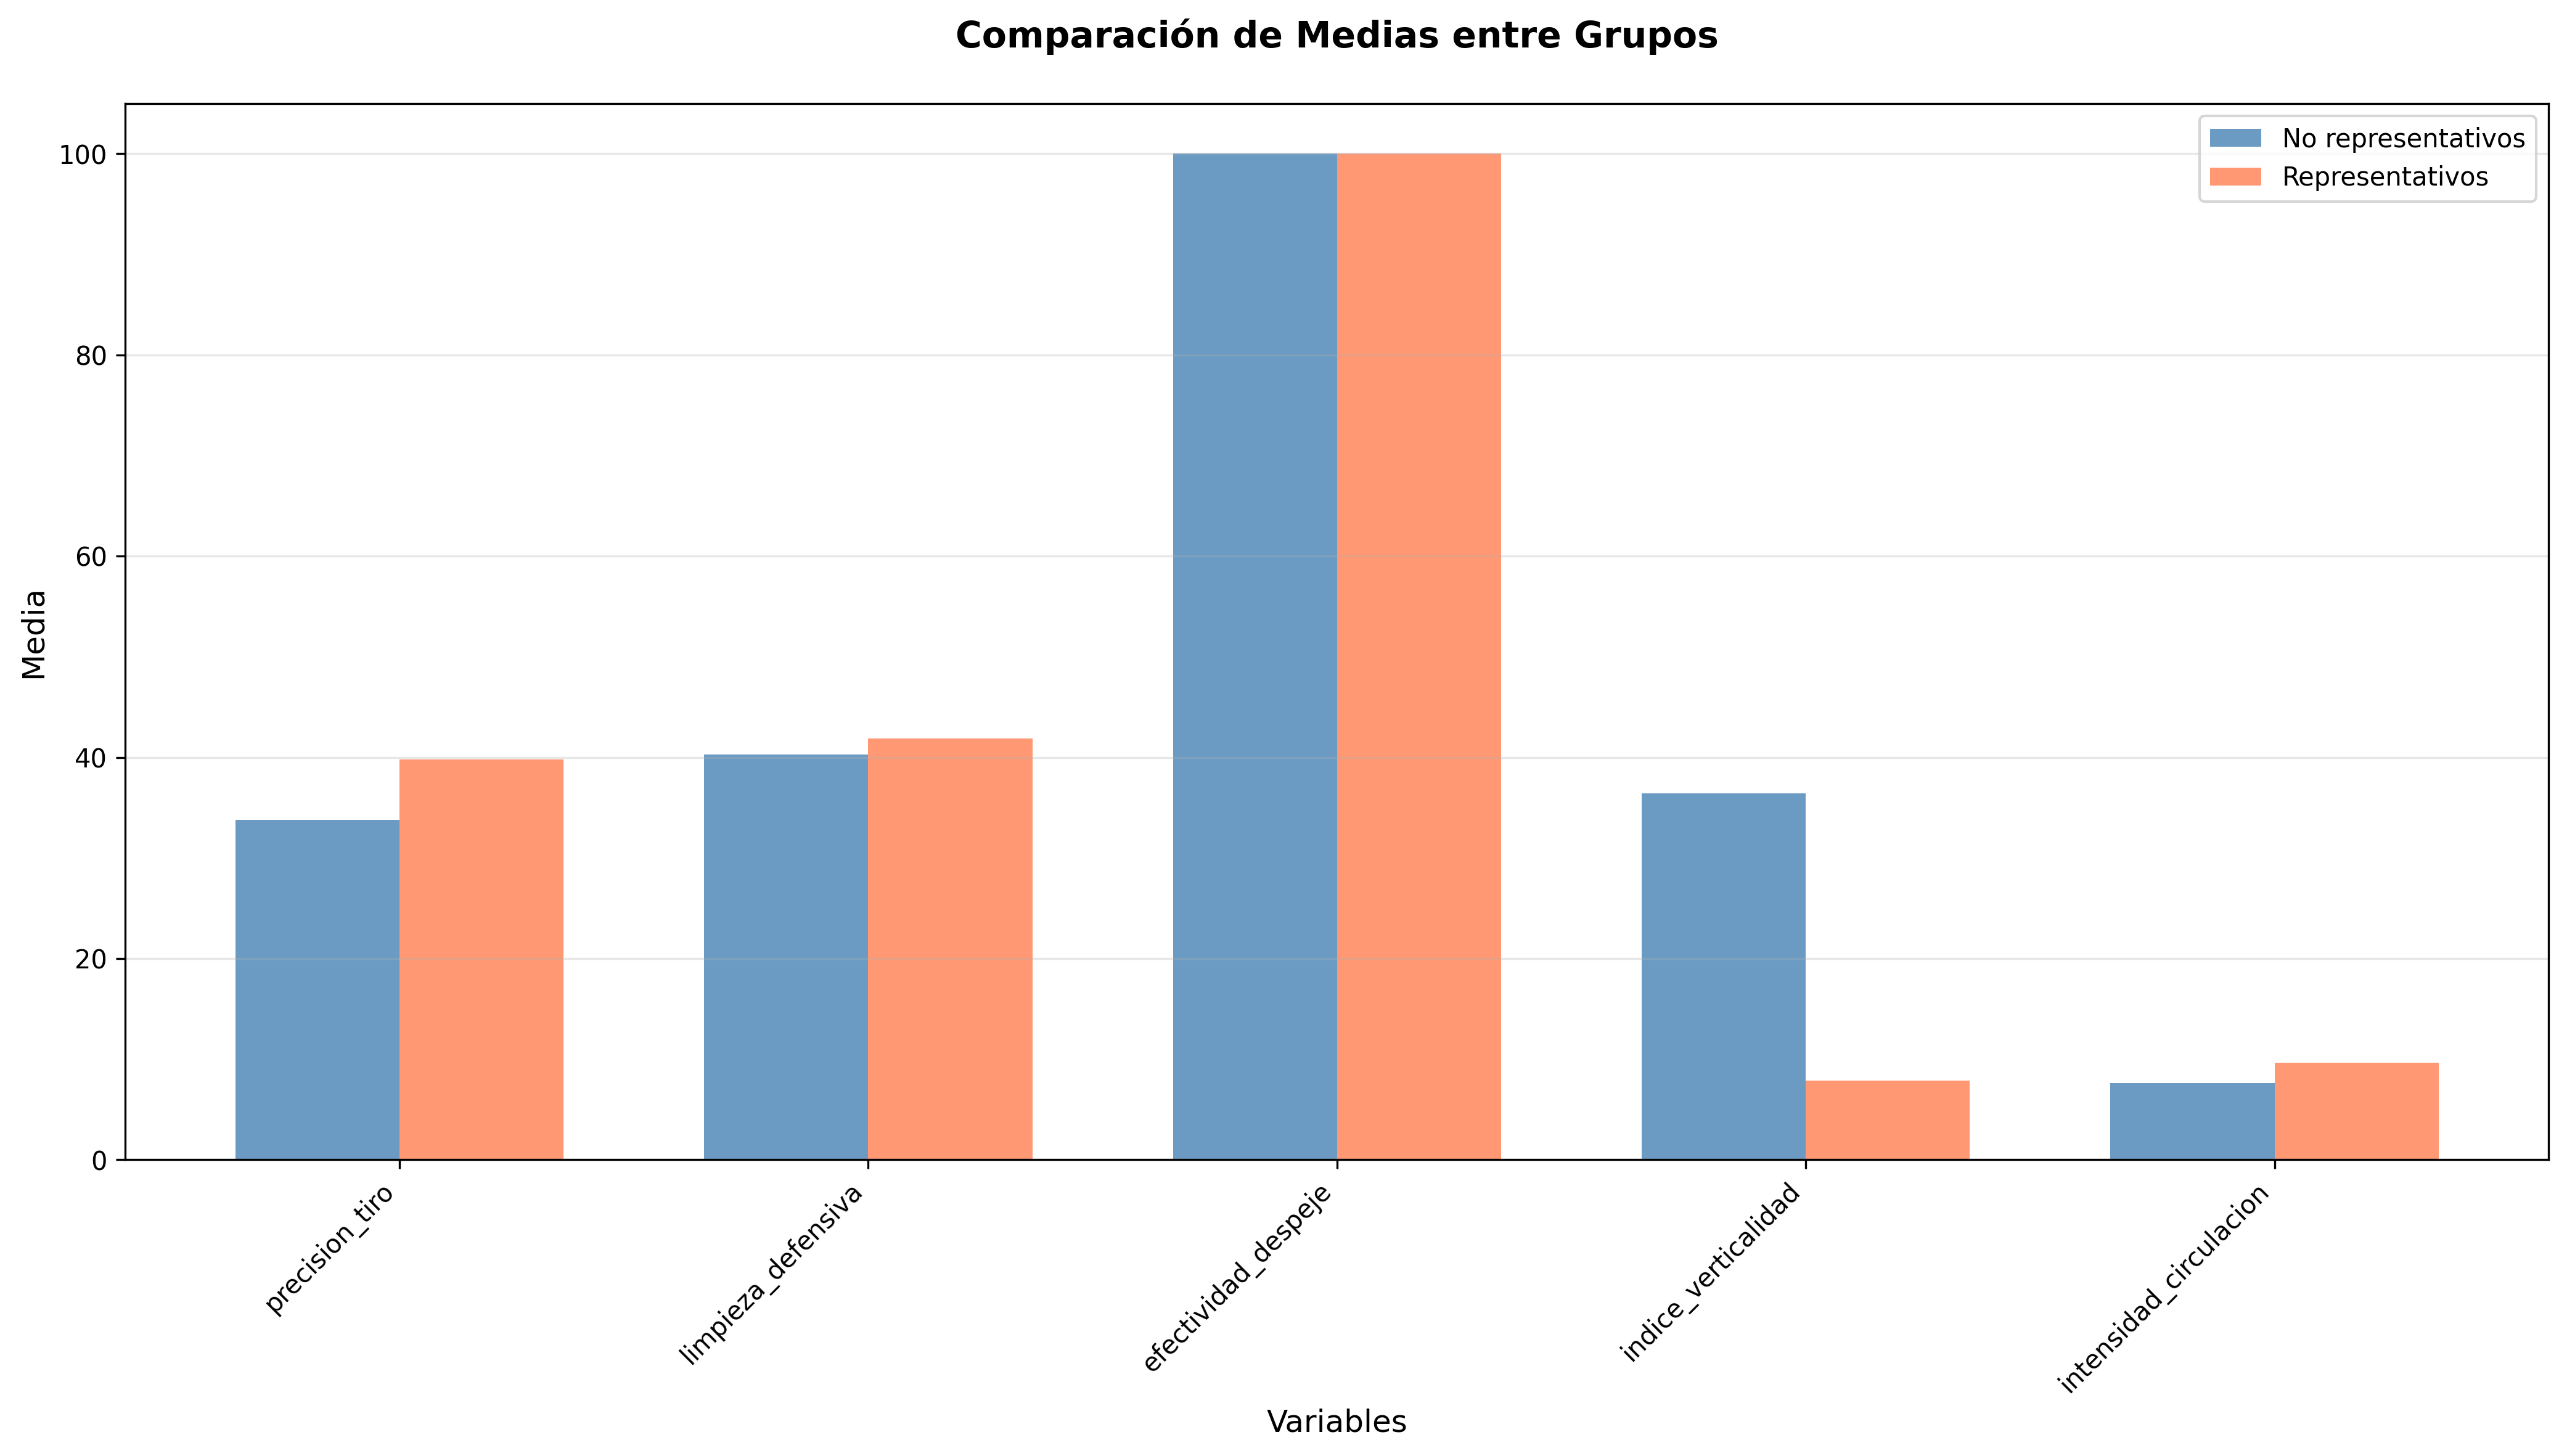
\includegraphics[width=0.9\textwidth]{NOTEBOOKS/comparison_barplot_large_scale.png}
		\caption{Variables de escala grande}
	\end{figure}
	
	\begin{figure}[H]
		\centering
		\begin{subfigure}{0.48\textwidth}
			\centering
			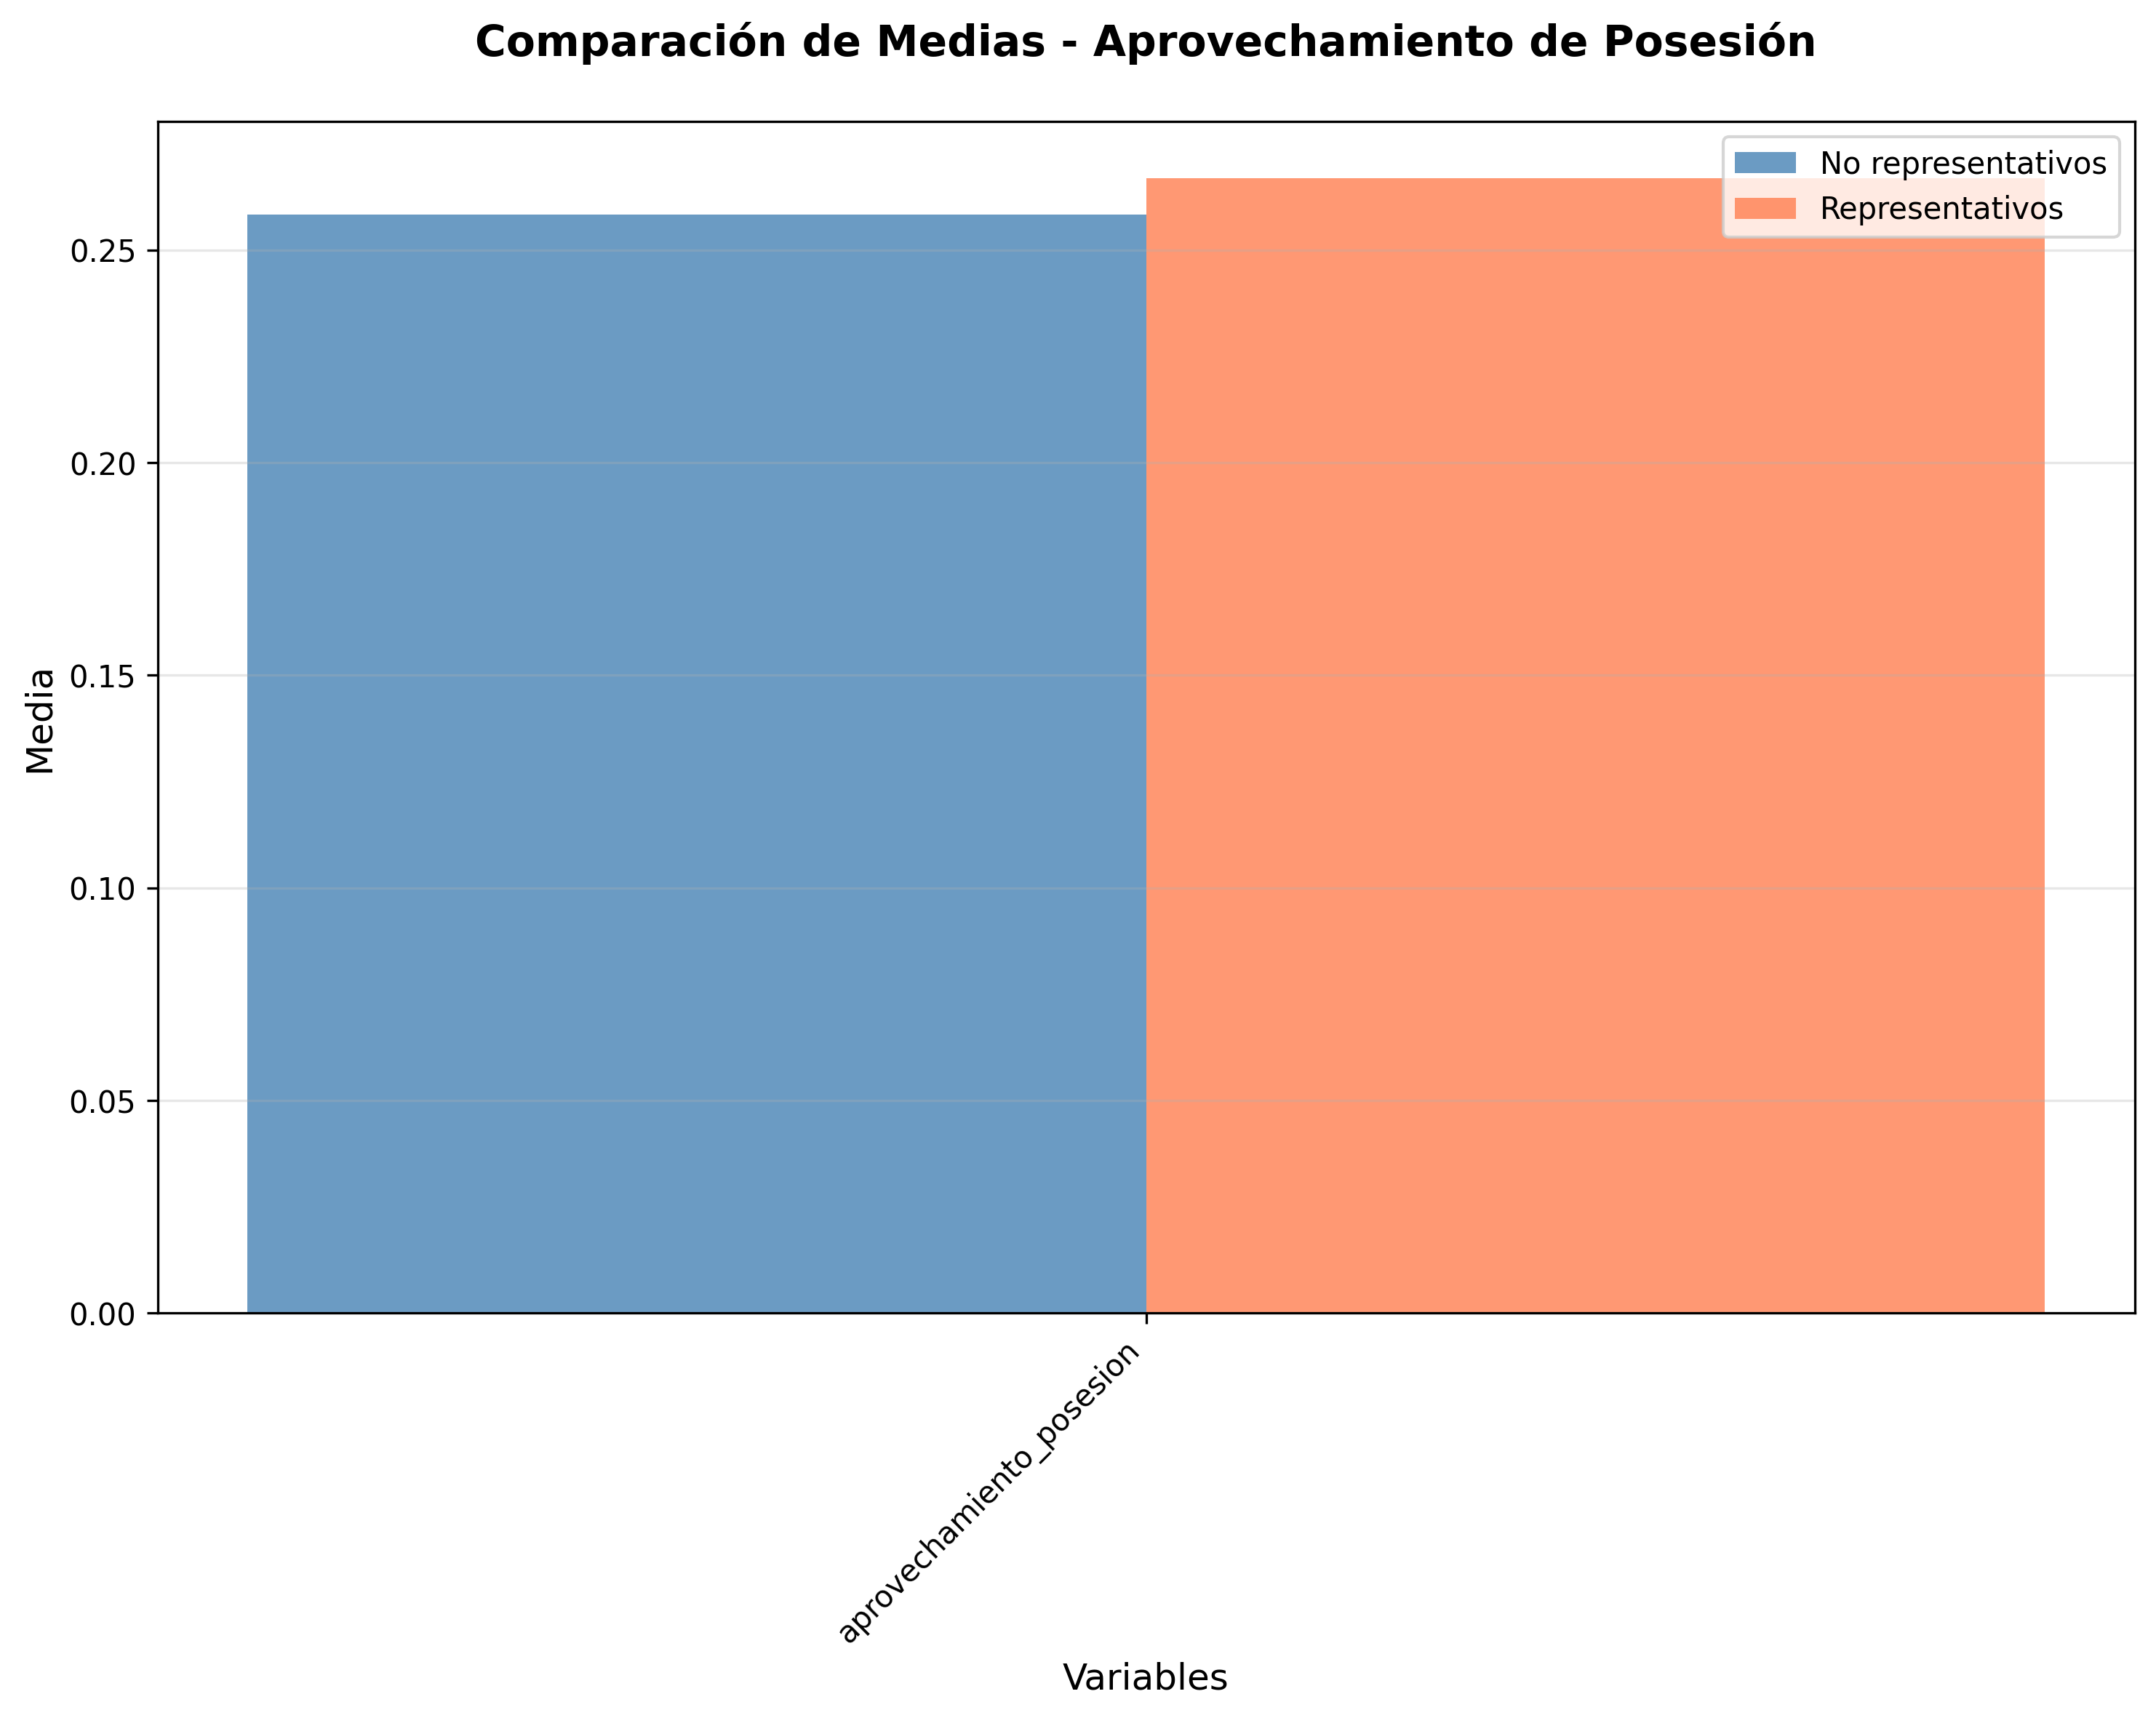
\includegraphics[width=\textwidth]{NOTEBOOKS/comparison_barplot_aprovechamiento.png}
			\caption{Aprovechamiento de posesión}
			\label{fig:aprovechamiento}
		\end{subfigure}
		\hfill
		\begin{subfigure}{0.48\textwidth}
			\centering
			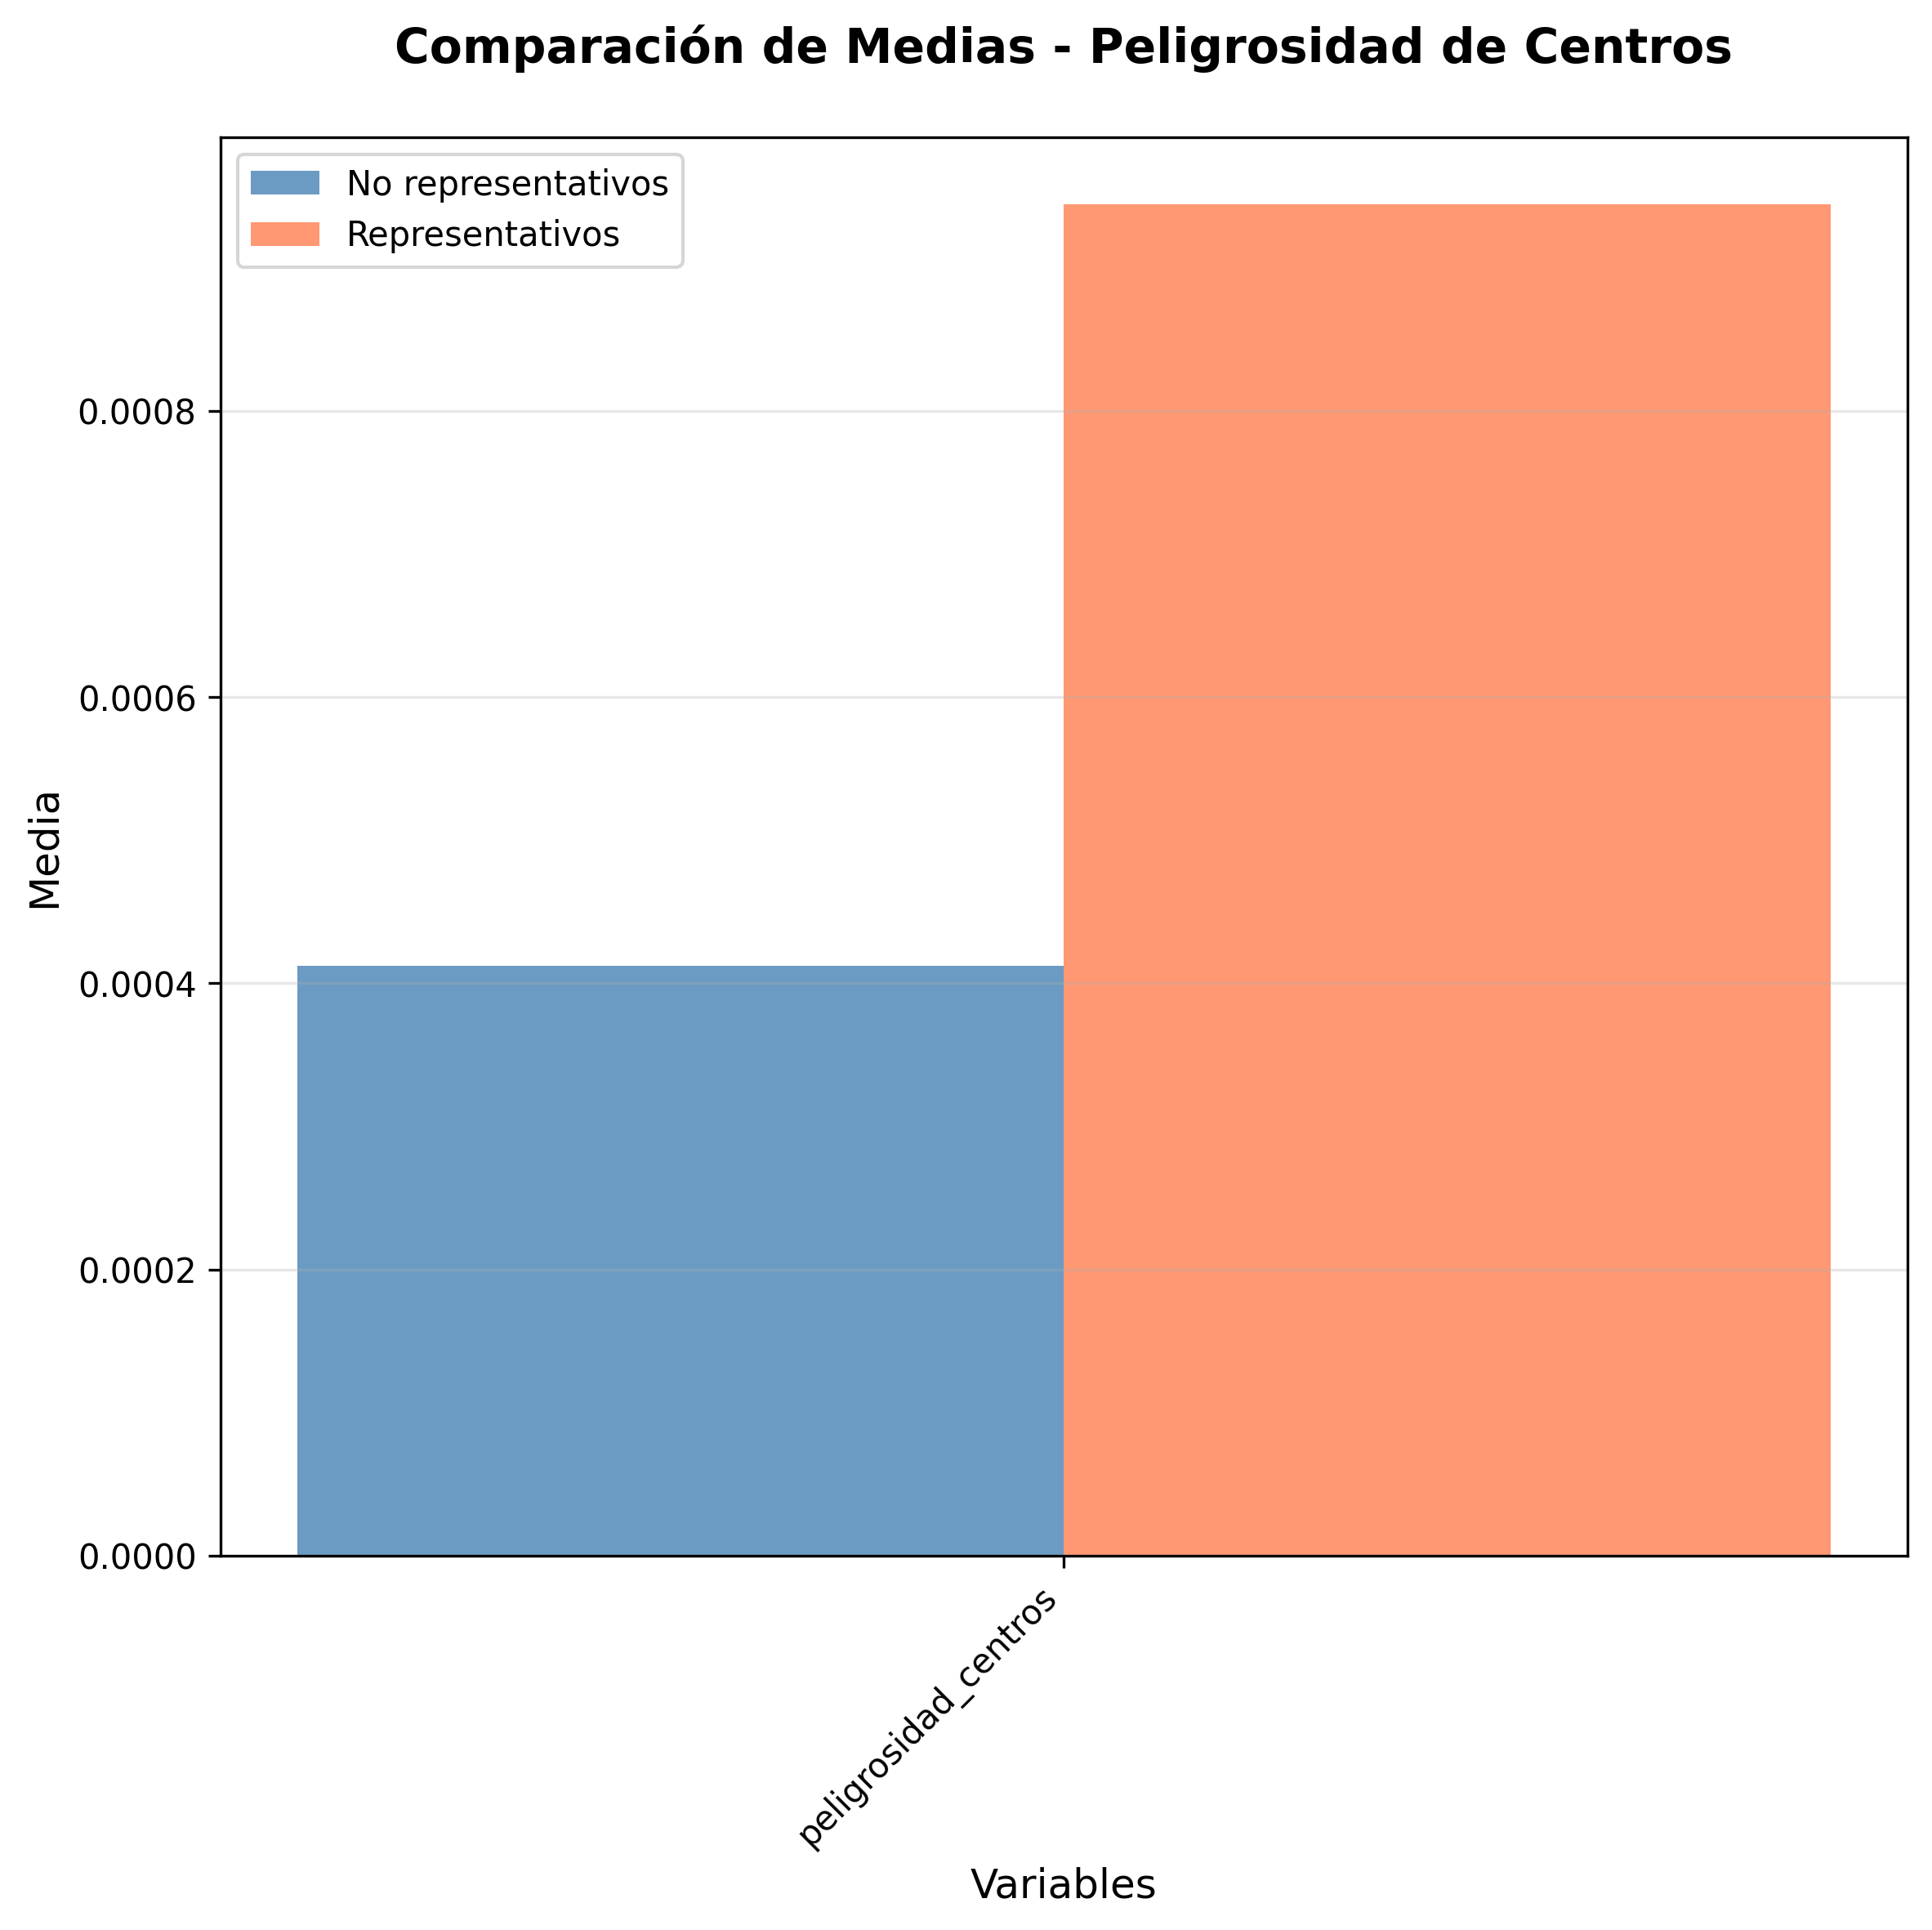
\includegraphics[width=\textwidth]{NOTEBOOKS/comparison_barplot_peligrosidad.png}
			\caption{Peligrosidad de centros}
			\label{fig:peligrosidad}
		\end{subfigure}
		\caption{Comparación de variables de escala pequeña}
		\label{fig:small_scale}
	\end{figure}
	A demás de las comparaciones que se pueden apreciar visualmente mediante los graficos de barras antes presentados, en la siguiente tabla se realizó una prueba t-Student de los KPIs definidos, en ella se puede apreciar una diferencia estadisticamente significativa entre ambos grupos nuevamente en cuanto a Precisión de Tiro, Peligrosidad de Centros, Limpieza Defensiva, Indice de Verticalidad e Intensidad de Circulación
	\newpage
	\vspace*{1cm}
	\begin{table}
\caption{Resultados completos de la prueba t-Student}
\label{tab:ttest_complete}
\resizebox{\textwidth}{!}{%
\begin{tabular}{lrrrrrrrrrr}
\toprule
Variable & Mean no rep & Std no rep & Mean rep & Std rep & Difference & n no rep & n rep & t statistic & p value & Significant \\
\midrule
precision tiro & 33.800000 & 16.002000 & 39.775000 & 14.780000 & 5.975000 & 609 & 872 & -7.398000 & 0.000000 & Si \\
aprovechamiento posesion & 0.258000 & 0.102000 & 0.267000 & 0.094000 & 0.008000 & 609 & 872 & -1.630000 & 0.103400 & No \\
peligrosidad centros & 0.000000 & 0.001000 & 0.001000 & 0.001000 & 0.001000 & 609 & 872 & -16.410000 & 0.000000 & Si \\
limpieza defensiva & 40.265000 & 12.639000 & 41.856000 & 12.907000 & 1.592000 & 609 & 872 & -2.355000 & 0.018600 & Si \\
efectividad despeje & 100.000000 & 0.000000 & 100.000000 & 0.000000 & 0.000000 & 609 & 872 & NaN & NaN & No \\
indice verticalidad & 36.440000 & 414.888000 & 7.877000 & 3.327000 & -28.563000 & 609 & 872 & 2.033000 & 0.042200 & Si \\
intensidad circulacion & 7.615000 & 1.960000 & 9.638000 & 1.114000 & 2.024000 & 609 & 872 & -25.212000 & 0.000000 & Si \\
\bottomrule
\end{tabular}
}
\end{table}
	

	\begin{small}
		{Todo el proceso detallado de estudio que fue realizado para llegar a las conclusiones presentadas puede ser visualizado através del siguiente enlace \url{https://github.com/kimachd/ESTADISTICA_sem_II_2025/tree/main}/}\\[2cm]
	\end{small}
	

	
	

	
	\end{document}